%%%%%%%%%%%%%%%%%%%%%%%%%%%%%%%%%%%%%%%%%%%%%%%%%%%%%%%%%%%%%%%%%%%%%%%%
%                                                                      %
%     File: Methodology/02_SystemControl.tex                           %
%     Tex Master: ../Thesis.tex                                        %
%                                                                      %
%%%%%%%%%%%%%%%%%%%%%%%%%%%%%%%%%%%%%%%%%%%%%%%%%%%%%%%%%%%%%%%%%%%%%%%%

\section{System Control}
\label{sec:system_control}
\label{chapter:control}

Having established, in Chapter~\ref{chapter:modeling}, the kinematic and dynamic models governing the USV and UAV, the natural next step is to determine how these models can be exploited to compute the control inputs that drive each vehicle along a desired trajectory. Because the two vehicles are physically coupled through the tether, their motion cannot be planned independently without accounting for this interaction, motivating a cooperative control strategy.

The overall control approach is therefore established first, followed by the design of the controllers for each vehicle.

\subsection{Cooperative Control Design}
\label{sec:ctrl_architecture}
Before formulating either controller, the strategies available are weighed against the system's dynamics and its objectives, so that the method chosen suits both vehicles.

\subsubsection{Control Method}
\label{sec:ctrl_method}

Keeping the tether within safe operating conditions depends on how the distance between the two vehicles evolves over time. A controller that only reacts to the current state can correct a violation only after it happens. Anticipating where the system is headed allows corrective action before reaching the safety limits.

A predictive controller does this by repeatedly solving, at each control instant, an optimization problem over a finite look-ahead window. Because the optimization runs over the predicted trajectory rather than the current state alone, requirements such as keeping the tether within safe conditions can be stated as explicit constraints in the problem itself, enforcing them explicitly over the prediction horizon.

The predictions rely on the model of the system dynamics, so their accuracy is tied to how well that model represents the real behaviour. The USV and UAV models derived in Chapter~\ref{chapter:modeling} include nonlinear terms. The predictive controller uses these nonlinear models directly, making non-linear model predictive control the method used for both vehicles.


\subsubsection{Cooperative Architecture}
\label{sec:ctrl_coop_architecture}

The USV and the UAV operate on different timescales. The \gls{usv} moves in the horizontal plane with slow, inertia-dominated motion. The \gls{uav}'s dynamics evolve much faster and demand a finer sampling time. A single \gls{nmpc} built around the combined state of both vehicles would force one prediction horizon and one sampling time onto both, compromising one vehicle's timescale to accommodate the other.

Combining both vehicles into one \gls{nmpc} would also enlarge the state, input, and constraint sets a single solver must handle, making a problem that already runs under real-time constraints harder to solve within the available computation time. Keeping the two problems separate matches each optimization's size to its own vehicle and keeps the computation more manageable in real time.

Each vehicle is therefore controlled by its own \gls{nmpc}. This separation isolates the two controllers from each other's failures: if one solver fails to find a feasible solution, the other vehicle's \gls{nmpc} continues operating on its own well-posed problem.

The tether's safety limits depend on the relative position between the USV and the UAV, so each vehicle's \gls{nmpc} accounts for the other vehicle's position. At every control instant, each controller receives the other vehicle's most recently computed predicted trajectory, and uses it to compute the predicted inter-vehicle distance at the nodes of its own horizon covered by that trajectory. Because the two controllers operate at different sampling intervals, the received predicted trajectory is temporally interpolated and resampled at the receiver's own prediction nodes.

Without this exchange, a vehicle would have to treat the other as stationary or extrapolate its motion from the last known state. Either assumption misrepresents the tether coupling and can drive the system into a constraint violation.

Because the \gls{uav} operates with a finer sampling time and a possibly shorter prediction horizon than the \gls{usv}, its predicted trajectory may cover only part of the \gls{usv}'s horizon. The \gls{usv} therefore enforces the tether constraint only at the nodes covered by the received trajectory, and leaves it inactive at the remaining ones, where no information about the \gls{uav} is available. This avoids constraining the \gls{usv} with an assumed \gls{uav} position that has no basis in the prediction. Since the problem is solved again at every instant, the covered window slides forward with time, and any potential violation is accounted for as soon as it enters it. In the opposite direction no such restriction is needed, since the \gls{usv}'s horizon fully covers that of the \gls{uav}.

Figure~\ref{fig:ctrl_architecture} shows this architecture, with two independent \gls{nmpc} loops, each driving its own vehicle, exchanging predicted horizons to enforce the tether constraint.

\begin{figure}[H]
    \centering
    \definecolor{okiBlue}{rgb}{0.0,0.447,0.698}
    \definecolor{okiGreen}{rgb}{0.0,0.620,0.451}
    \definecolor{okiVermillion}{rgb}{0.835,0.369,0.0}

    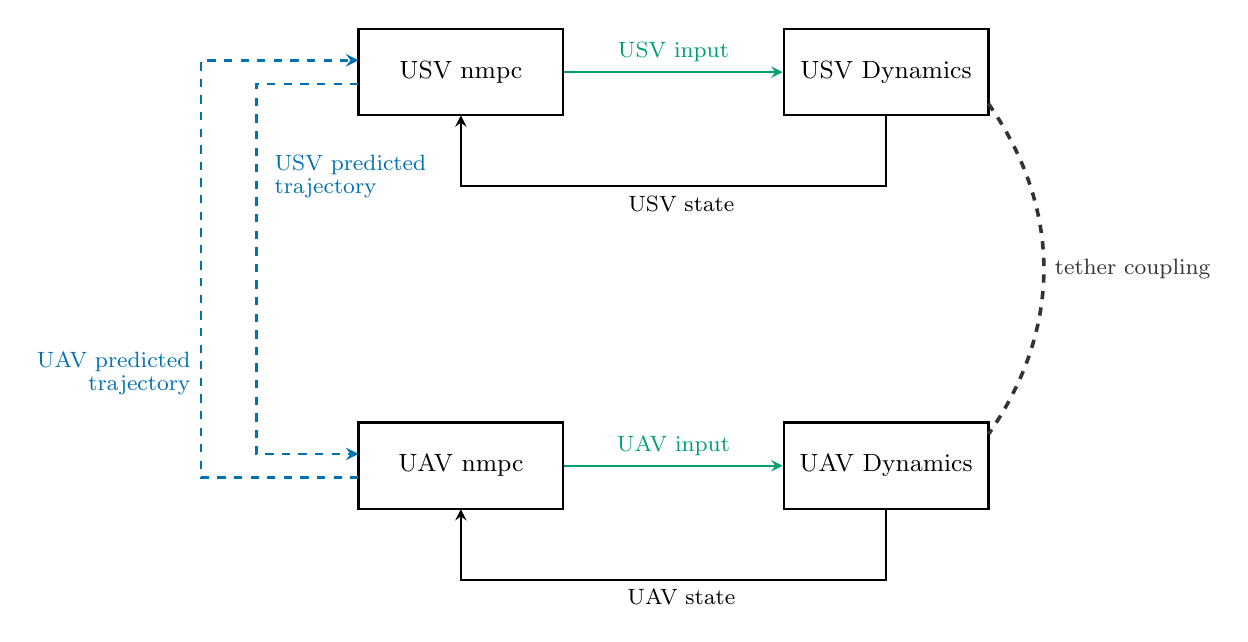
\begin{tikzpicture}[
        >=stealth,
        every node/.style={font=\small},
        boxStyle/.style={draw, rectangle, minimum height=1.1cm, minimum width=2.6cm, align=center, thick},
        sigArrow/.style={->, black, thick},
        exArrow/.style={->, okiBlue, dashed, line width=1.0pt},
        tetherStyle/.style={black!80, dashed, line width=1.3pt}
    ]

        % ---------- USV loop (top) ----------
        \node[boxStyle] (usvnmpc) at (0,5) {USV \gls{nmpc}};
        \node[boxStyle] (usvplant) at (5.4,5) {USV Dynamics};

        \draw[->, okiGreen, thick] (usvnmpc) -- (usvplant)
            node[midway, above, font=\footnotesize] {USV input};

        \draw[sigArrow] (5.4,4.45) -- (5.4,3.55) -- (0,3.55) -- (0,4.45);
        \node[below, font=\footnotesize] at (2.8,3.55) {USV state};

        % ---------- UAV loop (bottom) ----------
        \node[boxStyle] (uavnmpc) at (0,0) {UAV \gls{nmpc}};
        \node[boxStyle] (uavplant) at (5.4,0) {UAV Dynamics};

        \draw[->, okiGreen, thick] (uavnmpc) -- (uavplant)
            node[midway, above, font=\footnotesize] {UAV input};

        \draw[sigArrow] (5.4,-0.55) -- (5.4,-1.45) -- (0,-1.45) -- (0,-0.55);
        \node[below, font=\footnotesize] at (2.8,-1.45) {UAV state};

        % ---------- Coordination exchange between the two NMPCs ----------
        \draw[exArrow] (-1.3,4.85) -- (-2.6,4.85) -- (-2.6,0.15)
            node[pos=0.25, right, align=left, font=\footnotesize, xshift=0.1cm]
            {USV predicted\\[-1pt] trajectory}
            -- (-1.3,0.15);

        \draw[exArrow] (-1.3,-0.15) -- (-3.3,-0.15) -- (-3.3,5.15)
            node[pos=0.25, left, align=right, font=\footnotesize]
            {UAV predicted\\[-1pt] trajectory}
            -- (-1.3,5.15);

        % ---------- Physical tether coupling between plants ----------
        \draw[tetherStyle] (6.7,4.6) to[bend left=35]
            node[midway, right, font=\footnotesize] {tether coupling} (6.7,0.4);

    \end{tikzpicture}
    \caption{Cooperative control architecture diagram.}
    \label{fig:ctrl_architecture}
\end{figure}

\subsection{Nonlinear Model Predictive Control}
\label{sec:ctrl_nmpc_principles}

The vehicle models of Chapter~\ref{chapter:modeling} are continuous-time systems of the form
\begin{equation}
    \dot{\mathbf{x}} = \mathbf{f}\left( \mathbf{x}, \mathbf{u} \right),
    \label{eq:nmpc_dynamics_continuous}
\end{equation}
where $\mathbf{x} \in \mathbb{R}^{n_x}$ is the state vector and $\mathbf{u} \in \mathbb{R}^{n_u}$ is the control input vector.

However, the controller acts at discrete sampling instants $t_k = k T_s$, with the input held constant over each interval $[t_k, t_{k+1})$. Under this assumption, the state at the next instant follows from integrating the dynamics over one sampling interval,
\begin{equation}
    \mathbf{x}(t_{k+1}) = \mathbf{x}(t_k) + \int_{t_k}^{t_{k+1}} \mathbf{f}\left( \mathbf{x}(\tau), \mathbf{u}_k \right) d\tau.
    \label{eq:nmpc_dynamics_integral}
\end{equation}
Since this integral generally has no closed-form solution for nonlinear dynamics, it is approximated by applying a numerical integration scheme to $\mathbf{f}$ over one sampling interval. This defines a one-step discrete map $\boldsymbol\Phi$,
\begin{equation}
    \mathbf{x}_{k+1} = \boldsymbol\Phi\left( \mathbf{x}_k, \mathbf{u}_k \right),
    \label{eq:nmpc_dynamics_general}
\end{equation}
where $\mathbf{x}_k \approx \mathbf{x}(t_k)$ is the system state at instant $k$, so that $\boldsymbol\Phi$ returns the approximate state one sampling interval ahead, given the current state and input.

At every instant $k$, \gls{nmpc} uses this map to predict the future behaviour of the system over a finite look-ahead window of $N$ steps, and computes the input that steers it toward a reference. Denote by $\hat{\mathbf{x}}_{k+i|k}$ and $\hat{\mathbf{u}}_{k+i|k}$ the state and input predicted $i$ steps ahead at instant $k$, for $i = 0, \dots, N$ and $i = 0, \dots, N-1$, respectively. The predicted trajectory starts from the estimated current state,
\begin{equation}
    \hat{\mathbf{x}}_{k|k} = \mathbf{x}_k,
    \label{eq:nmpc_x0}
\end{equation}
and evolves according to the system model,
\begin{equation}
    \hat{\mathbf{x}}_{k+i+1|k} = \boldsymbol\Phi\left( \hat{\mathbf{x}}_{k+i|k}, \hat{\mathbf{u}}_{k+i|k} \right), \quad i = 0, \dots, N-1.
    \label{eq:nmpc_prediction}
\end{equation}

Each predicted step is then scored against a reference trajectory. A stage cost $\ell(\hat{\mathbf{x}}_{k+i|k}, \hat{\mathbf{u}}_{k+i|k})$, typically quadratic, penalizes the tracking error and the control effort at every step of the horizon, and a terminal cost $\ell_f(\hat{\mathbf{x}}_{k+N|k})$ penalizes the tracking error at its final step. Summing both over the horizon gives the total predicted cost,
\begin{equation}
    J = \sum_{i=0}^{N-1} \ell\left( \hat{\mathbf{x}}_{k+i|k}, \hat{\mathbf{u}}_{k+i|k} \right) + \ell_f\left( \hat{\mathbf{x}}_{k+N|k} \right).
    \label{eq:nmpc_cost}
\end{equation}

Minimizing $J$ alone ignores the physical limits of the system, so the prediction is also constrained. The predicted states and inputs must remain within the admissible sets $\mathcal{X}$ and $\mathcal{U}$ at every step of the horizon,
\begin{align}
    \hat{\mathbf{x}}_{k+i|k} &\in \mathcal{X}, \quad i = 0, \dots, N, \label{eq:nmpc_bounds_x} \\
    \hat{\mathbf{u}}_{k+i|k} &\in \mathcal{U}, \quad i = 0, \dots, N-1, \label{eq:nmpc_bounds_u}
\end{align}
where $\mathcal{X}$ and $\mathcal{U}$ collect the admissible states and inputs. These sets may be defined by simple bounds or by general nonlinear inequality constraints of the form $h(\hat{\mathbf{x}}_{k+i|k}, \hat{\mathbf{u}}_{k+i|k}) \le 0$.

Enforcing these sets as hard constraints can make the problem infeasible. If a disturbance pushes the true state outside the admissible set, no predicted trajectory satisfies the constraints, and the solver has no solution to return even though one is required at every sampling instant. To avoid this, a constraint $h(\hat{\mathbf{x}}_{k+i|k}, \hat{\mathbf{u}}_{k+i|k}) \le 0$ can be softened by a slack variable $\sigma \ge 0$,
\begin{equation}
    h(\hat{\mathbf{x}}_{k+i|k}, \hat{\mathbf{u}}_{k+i|k}) \le \sigma,
    \label{eq:nmpc_soft_constraint}
\end{equation}
which allows the constraint to be violated by an amount $\sigma$. The slack becomes an additional decision variable at each step where the constraint is softened, and a penalty
\begin{equation}
    \rho(\sigma) = \mu_{1}\sigma + \mu_{2}\sigma^2, \qquad \mu_{1}, \mu_{2} \ge 0,
    \label{eq:nmpc_slack_penalty}
\end{equation}
is added to the cost $J$ for each slack. Since $\rho(0) = 0$, the solver prefers $\sigma = 0$ whenever the original constraint can be met, and large weights $\mu_1, \mu_2$ keep any violation close to zero.

Assembling the cost, the prediction model, and the constraints defines the optimal control problem solved at every sampling instant $k$,
\begin{align}
    \min_{\hat{\mathbf{x}}_{k+i|k}, \, \hat{\mathbf{u}}_{k+i|k}, \, \hat{\sigma}_{k+i|k}} \quad & J + \sum_{i=0}^{N-1} \rho\left( \hat{\sigma}_{k+i|k} \right) \label{eq:nmpc_ocp_cost} \\
    \text{s.t.} \quad & \hat{\mathbf{x}}_{k|k} = \mathbf{x}_k, \notag \\
    & \hat{\mathbf{x}}_{k+i+1|k} = \boldsymbol\Phi\left( \hat{\mathbf{x}}_{k+i|k}, \hat{\mathbf{u}}_{k+i|k} \right), \quad i = 0, \dots, N-1, \notag \\
    & \hat{\mathbf{x}}_{k+i|k} \in \mathcal{X}, \quad i = 0, \dots, N, \notag \\
    & \hat{\mathbf{u}}_{k+i|k} \in \mathcal{U}, \quad i = 0, \dots, N-1, \notag \\
    & h\left( \hat{\mathbf{x}}_{k+i|k}, \hat{\mathbf{u}}_{k+i|k} \right) \le \hat{\sigma}_{k+i|k}, \quad \hat{\sigma}_{k+i|k} \ge 0, \quad i = 0, \dots, N-1. \notag
\end{align}

Solving this problem returns a full predicted input sequence, $\hat{\mathbf{u}}_{k|k}, \dots, \hat{\mathbf{u}}_{k+N-1|k}$, but only its first element, $\hat{\mathbf{u}}_{k|k}$, is applied to the system. At the next instant, $k+1$, the state is estimated again and the problem is solved again from $\hat{\mathbf{x}}_{k+1|k+1} = \mathbf{x}_{k+1}$, with the horizon shifted one step forward. This strategy, known as the receding horizon principle, computes every input from the latest state estimate, so the controller can correct for disturbances and model errors that the previous prediction did not anticipate.


\subsection{USV NMPC}
\label{sec:ctrl_usv_mpc}

The USV NMPC computes, at every sampling instant, the thruster commands that best track a reference trajectory over a finite prediction horizon, subject to the vessel's dynamics, the physical limits of its actuators, and the tether workspace. It predicts the vessel's motion with the model derived in Chapter~\ref{chapter:modeling}, and solves a constrained optimization problem at each step to obtain the commands applied to the thrusters.

\subsubsection*{Predictive Model}

The vessel model of Chapter~\ref{chapter:modeling} is driven by the resultant thrust force and moment $\boldsymbol\tau = [X,Y,N]^\top$, which are obtained from the physical actuator commands $T_L, T_R, \alpha_L, \alpha_R$ through the allocation
\begin{equation}
    X = T_L\cos\alpha_L + T_R\cos\alpha_R, \qquad Y = T_L\sin\alpha_L + T_R\sin\alpha_R,
    \label{eq:usv_mpc_alloc_force}
\end{equation}
\begin{equation}
    N = -x_{arm}\big(T_L\sin\alpha_L+T_R\sin\alpha_R\big) - y_{arm}\big(T_L\cos\alpha_L-T_R\cos\alpha_R\big).
    \label{eq:usv_mpc_alloc_moment}
\end{equation}

Since the controller ultimately has to command $T_L, T_R, \alpha_L, \alpha_R$, the \gls{nmpc} is formulated directly in terms of these variables, rather than choosing $\boldsymbol\tau$ and allocating it separately. This way, the limits of the physical actuators can be imposed directly in the optimization problem.

Each thruster is limited both in the thrust and azimuth it can deliver,
\begin{equation}
    T_{L,min} \le T_L \le T_{L,max}, \quad T_{R,min} \le T_R \le T_{R,max}, \quad \alpha_{L,min} \le \alpha_L \le \alpha_{L,max}, \quad \alpha_{R,min} \le \alpha_R \le \alpha_{R,max},
    \label{eq:usv_mpc_state_bounds}
\end{equation}
and in how fast it can change them,
\begin{equation}
    |\dot{T}_L| \le \dot{T}_{L,max}, \quad |\dot{T}_R| \le \dot{T}_{R,max}, \quad |\dot{\alpha}_L| \le \dot{\alpha}_{L,max}, \quad |\dot{\alpha}_R| \le \dot{\alpha}_{R,max}.
    \label{eq:usv_mpc_input_bounds}
\end{equation}
The rate limits act on the time derivatives of the commands, so imposing them directly as bounds requires these derivatives to become the control input,
\begin{equation}
    \mathbf{u}_v = [\dot{T}_L, \dot{T}_R, \dot{\alpha}_L, \dot{\alpha}_R]^\top \in \mathbb{R}^4,
    \label{eq:usv_mpc_input_augmented}
\end{equation}
which in turn makes $T_L, T_R, \alpha_L, \alpha_R$ part of the state vector,
\begin{equation}
    \mathbf{x}_v = [x, y, \psi, u, v, r,\ T_L, T_R, \alpha_L, \alpha_R]^\top \in \mathbb{R}^{10}.
    \label{eq:usv_mpc_state_augmented}
\end{equation}
With this choice, the range limits act on the state, and the rate limits act directly on the input.

With $\mathbf{x}_v$ and $\mathbf{u}_v$ defined, the prediction model $\dot{\mathbf{x}}_v = \mathbf{f}_v(\mathbf{x}_v,\mathbf{u}_v)$ is assembled from the vessel kinematics and dynamics.

The kinematics are given by \eqref{eq:usv_kinematics_planar} and \eqref{eq:usv_psi_dot},
\begin{equation}
    \dot x = u\cos\psi - v\sin\psi, \qquad \dot y = u\sin\psi + v\cos\psi, \qquad \dot\psi = r.
    \label{eq:usv_mpc_kinematics}
\end{equation}

The dynamics follow \eqref{eq:usv_udot}--\eqref{eq:usv_rdot}, with $X,Y,N$ given by \eqref{eq:usv_mpc_alloc_force}--\eqref{eq:usv_mpc_alloc_moment} in terms of the thruster state,
\begin{equation}
    \dot u = \frac{1}{m}\Big[X - \big(X_u+X_{uu}^{\pm}|u|\big)u\Big] + vr,
    \label{eq:usv_mpc_udot}
\end{equation}
\begin{equation}
    \dot v = \frac{1}{m}\Big[Y - \big(Y_v+Y_{vv}|v|\big)v\Big] - ur,
    \label{eq:usv_mpc_vdot}
\end{equation}
\begin{equation}
    \dot r = \frac{1}{I_z}\Big[N - \big(N_r+N_{rr}|r|\big)r\Big].
    \label{eq:usv_mpc_rdot}
\end{equation}

Finally, $\dot T_L,\dot T_R,\dot\alpha_L,\dot\alpha_R$ appear directly as the components of $\mathbf{u}_v$,
\begin{equation}
    \dot T_L = \dot T_L, \qquad \dot T_R = \dot T_R, \qquad \dot\alpha_L = \dot\alpha_L, \qquad \dot\alpha_R = \dot\alpha_R.
    \label{eq:usv_mpc_thruster_rates}
\end{equation}

Discretization over a sampling interval $T_s$, following Section~\ref{sec:ctrl_nmpc_principles}, gives the one-step map $\boldsymbol\Phi_v$ such that $\hat{\mathbf{x}}_{v,k+i+1|k} = \boldsymbol\Phi_v\big(\hat{\mathbf{x}}_{v,k+i|k}, \hat{\mathbf{u}}_{v,k+i|k}\big)$ approximates the solution of $\dot{\mathbf{x}}_v = \mathbf{f}_v(\mathbf{x}_v,\mathbf{u}_v)$ over one sampling interval.


\subsubsection*{Cost and Constraints}
 
Let $\mathbf{p} = [x,y]^\top$ denote the position, $\psi$ the heading, and $\boldsymbol{\nu} = [u,v,r]^\top$ the body-fixed velocities, with $\mathbf{p}_{ref}$, $\psi_{ref}$, and $\boldsymbol{\nu}_{ref}$ the corresponding references from a given trajectory.

Tracking the reference position is penalized quadratically as
\begin{equation}
    \|\mathbf{p}-\mathbf{p}_{ref}\|^2_{Q_p},
    \label{eq:usv_mpc_cost_pos}
\end{equation}
where $\|\boldsymbol\xi\|^2_W \coloneqq \boldsymbol\xi^\top W \boldsymbol\xi$ for a positive semi-definite weighting matrix $W$, which sets the relative importance of each component of $\boldsymbol\xi$ in the cost.

Tracking the heading reference is penalized as
\begin{equation}
    q_\psi\big(1-\cos(\psi-\psi_{ref})\big),
    \label{eq:usv_mpc_cost_heading}
\end{equation}
where $q_\psi \ge 0$ is a scalar weight setting the relative importance of heading tracking.

Both $\psi$ and $\psi_{ref}$ are angles represented within an interval of width $2\pi$, such as $(-\pi,\pi]$. When they lie near opposite ends of this interval, their raw difference $\psi-\psi_{ref}$ approaches $\pm2\pi$, even though the two headings are then almost identical. As $\cos(\cdot)$ has period $2\pi$, its value approaches one whenever $\psi-\psi_{ref}$ is near zero or $\pm2\pi$, so the cost \eqref{eq:usv_mpc_cost_heading} is near zero in both cases, correctly reflecting that the two headings are almost identical.

Tracking the reference velocity is penalized in the same way as the position,
\begin{equation}
    \|\boldsymbol{\nu}-\boldsymbol{\nu}_{ref}\|^2_{Q_\nu}.
    \label{eq:usv_mpc_cost_vel}
\end{equation}

The thruster commands $T_L, T_R, \alpha_L, \alpha_R$ are regularized directly as
\begin{equation}
    \big\|[T_L,T_R,\alpha_L,\alpha_R]^\top\big\|^2_{Q_\tau},
    \label{eq:usv_mpc_cost_reg}
\end{equation}
discouraging thrust and azimuth commands larger than necessary to track the reference.

The last term penalizes $\mathbf{u}_v$, the rate of change of the thruster commands,
\begin{equation}
    \big\|[\dot{T}_L, \dot{T}_R, \dot{\alpha}_L, \dot{\alpha}_R]^\top\big\|^2_{R},
    \label{eq:usv_mpc_cost_rate}
\end{equation}
discouraging abrupt changes in thrust and azimuth between consecutive instants.

Summing \eqref{eq:usv_mpc_cost_pos}--\eqref{eq:usv_mpc_cost_rate} gives the stage cost
\begin{equation}
    \begin{aligned}
        \ell(\mathbf{x}_v, \mathbf{u}_v) = {} & \|\mathbf{p}-\mathbf{p}_{ref}\|^2_{Q_p} + q_\psi\big(1-\cos(\psi-\psi_{ref})\big) + \|\boldsymbol{\nu}-\boldsymbol{\nu}_{ref}\|^2_{Q_\nu} \\
        & + \big\|[T_L,T_R,\alpha_L,\alpha_R]^\top\big\|^2_{Q_\tau} + \big\|[\dot{T}_L, \dot{T}_R, \dot{\alpha}_L, \dot{\alpha}_R]^\top\big\|^2_{R}.
    \end{aligned}
    \label{eq:usv_mpc_stage_cost}
\end{equation}

The terminal cost $\ell_f$ penalizes the last predicted state, so that the optimizer does not disregard where the vessel ends up at the end of the horizon. It equals the stage cost \eqref{eq:usv_mpc_stage_cost} without the input rate term, since no control input is chosen at the final node:
\begin{equation}
    \ell_f(\mathbf{x}_v) = \|\mathbf{p}-\mathbf{p}_{ref}\|^2_{Q_p} + q_\psi\big(1-\cos(\psi-\psi_{ref})\big) + \|\boldsymbol{\nu}-\boldsymbol{\nu}_{ref}\|^2_{Q_\nu} + \big\|[T_L,T_R,\alpha_L,\alpha_R]^\top\big\|^2_{Q_\tau}.
    \label{eq:usv_mpc_terminal_cost}
\end{equation}
 
The thruster limits introduced in the predictive model enter the optimization problem as constraints. Since thrust and azimuth are components of the state, their range limits define the admissible state set
\begin{equation}
    \mathcal{X} = \left\{ \mathbf{x}_v : \;
    \begin{aligned}
        & T_{L,min} \le T_L \le T_{L,max}, \quad T_{R,min} \le T_R \le T_{R,max}, \\
        & \alpha_{L,min} \le \alpha_L \le \alpha_{L,max}, \quad \alpha_{R,min} \le \alpha_R \le \alpha_{R,max}
    \end{aligned}
    \right\},
    \label{eq:usv_mpc_set_X}
\end{equation}
while the limits on their rates of change, which act on the input, define the admissible input set
\begin{equation}
    \mathcal{U} = \left\{ \mathbf{u}_v : \;
    \begin{aligned}
        & |\dot{T}_L| \le \dot{T}_{L,max}, \quad |\dot{T}_R| \le \dot{T}_{R,max}, \\
        & |\dot{\alpha}_L| \le \dot{\alpha}_{L,max}, \quad |\dot{\alpha}_R| \le \dot{\alpha}_{R,max}
    \end{aligned}
    \right\}.
    \label{eq:usv_mpc_set_U}
\end{equation}

The last constraint couples the vessel to the UAV through the tether, and is the only one that depends on the other vehicle. The tether limits the distance between its attachment point on the vessel deck and the UAV to a maximum admissible separation $d_{max}$. The attachment point is vertically aligned with the origin of the vessel's body frame, at a fixed height $z_t$ in the inertial frame, so its position is $(x, y, z_t)$. Along the horizon, the USV controller uses the UAV's most recently computed predicted trajectory $\hat{\mathbf{p}}_a = [\hat x_a, \hat y_a, \hat z_a]^\top$, temporally resampled at the vessel's prediction nodes covered by it, to compute the squared distance between the attachment point and the UAV,
\begin{equation}
    d^2 = (x - \hat x_a)^2 + (y - \hat y_a)^2 + (\hat z_a - z_t)^2.
    \label{eq:usv_mpc_tether_distance}
\end{equation}
The requirement $d^2 \le d_{max}^2$ is enforced as a soft constraint through a slack variable $\sigma \ge 0$,
\begin{equation}
    \underbrace{d^2 - d_{max}^2}_{h(\mathbf{x}_v)} \le \sigma,
    \label{eq:usv_mpc_tether_constraint}
\end{equation}
which is penalized by $\rho(\sigma)$ as in \eqref{eq:nmpc_slack_penalty}, with large weights $\mu_1$ and $\mu_2$ so that violations remain small whenever geometrically feasible.

\subsubsection*{Optimal Control Problem}
 
At every sampling instant $k$, the kinematic and dynamic components of the initial state come from the vessel's current estimate, while the thruster components use the last command actually applied:
\begin{equation}
    \mathbf{x}_{v,k} = \big[x_k, y_k, \psi_k, u_k, v_k, r_k,\ T_{L,k-1}, T_{R,k-1}, \alpha_{L,k-1}, \alpha_{R,k-1}\big]^\top.
    \label{eq:usv_mpc_initial_condition}
\end{equation}
Starting from the last applied command ensures that the rate limits in \eqref{eq:usv_mpc_input_bounds} are enforced relative to the actual thruster values, so the first input chosen is always attainable by the thrusters.

The references and the \gls{uav}'s predicted trajectory are given data at each instant. Since the \gls{uav}'s predicted trajectory can be shorter than the vessel's horizon, let $N_c \le N$ denote the last node of the vessel's horizon covered by it. The tether constraint, and its slack, are enforced only for $i = 0, \dots, N_c$.
 
Assembling the cost, the model, and the constraints gives the optimal control problem the USV solves at every sampling instant:
\begin{align}
    \min_{\hat{\mathbf{x}}_v,\, \hat{\mathbf{u}}_v,\, \hat{\sigma}} \quad & \sum_{i=0}^{N-1} \ell\big(\hat{\mathbf{x}}_{v,k+i|k}, \hat{\mathbf{u}}_{v,k+i|k}\big) + \ell_f\big(\hat{\mathbf{x}}_{v,k+N|k}\big) + \sum_{i=0}^{N_c} \rho\big(\hat\sigma_{k+i|k}\big) \notag \\
    \text{s.t.} \quad & \hat{\mathbf{x}}_{v,k|k} = \mathbf{x}_{v,k}, \notag \\
    & \hat{\mathbf{x}}_{v,k+i+1|k} = \boldsymbol\Phi_v\big(\hat{\mathbf{x}}_{v,k+i|k}, \hat{\mathbf{u}}_{v,k+i|k}\big), \quad i = 0, \dots, N-1, \notag \\
    & \hat{\mathbf{x}}_{v,k+i|k} \in \mathcal{X}, \quad i = 0, \dots, N, \notag \\
    & \hat{\mathbf{u}}_{v,k+i|k} \in \mathcal{U}, \quad i = 0, \dots, N-1, \notag \\
    & h\big(\hat{\mathbf{x}}_{v,k+i|k}\big) \le \hat\sigma_{k+i|k}, \quad \hat\sigma_{k+i|k} \ge 0, \quad i = 0, \dots, N_c. \label{eq:usv_mpc_ocp}
\end{align}
The vessel's low-level actuators receive the integrated thruster commands $T_{L,k}, T_{R,k}, \alpha_{L,k}, \alpha_{R,k}$, obtained by integrating the first optimal input rate $\hat{\mathbf{u}}_{v,k|k}$ over the sampling interval $T_s$. These become the thruster components of the initial state at the subsequent sampling instant.
 
%%%%%%%%%%%%%%%%%%%%%%%%%%%%%%%%%%%%%%%%%%%%%%%%%%%%%%%%%%%%%%%%%%%%%%%%%%%%%%%%%%%%%%%%%
\subsection{UAV NMPC}
\label{sec:ctrl_uav_mpc}

The UAV NMPC computes, at every sampling instant, the thrust and attitude commands that best track a reference trajectory over a finite prediction horizon, subject to the vehicle's dynamics, its actuation limits, and the tether workspace. It predicts the vehicle's motion with the model derived in Chapter~\ref{chapter:modeling}, and solves a constrained optimization problem at each step to obtain the commands applied to the vehicle.

\subsubsection*{Predictive Model}

The input $\mathbf{u}_a = [T,\phi,\theta,\psi]^\top$ of the vehicle model defined in Chapter~\ref{chapter:modeling} commands the thrust and the attitude directly, assuming each of them is reached instantaneously.

Similarly to the thrusters of the USV, the attitude of the \gls{uav} cannot change arbitrarily fast, and its rate of change is limited,
\begin{equation}
    |\dot\phi| \le \dot\phi_{max}, \quad |\dot\theta| \le \dot\theta_{max}, \quad |\dot\psi| \le \dot\psi_{max}.
    \label{eq:uav_mpc_rate_bounds}
\end{equation}
Since these limits act on the time derivatives of the attitude, imposing them directly as bounds requires the rates to be part of the control input,
\begin{equation}
    \mathbf{u}_a = [\dot\phi,\dot\theta,\dot\psi,T]^\top \in \mathbb{R}^4,
    \label{eq:uav_mpc_input_augmented}
\end{equation}
which makes $\phi,\theta,\psi$ part of the state vector,
\begin{equation}
    \mathbf{x}_a = [x,y,z,\dot x,\dot y,\dot z,\ \phi,\theta,\psi]^\top \in \mathbb{R}^{9}.
    \label{eq:uav_mpc_state_augmented}
\end{equation}

With $\mathbf{x}_a$ and $\mathbf{u}_a$ defined, the prediction model $\dot{\mathbf{x}}_a = \mathbf{f}_a(\mathbf{x}_a,\mathbf{u}_a)$ is assembled from the \gls{uav} kinematics and dynamics, together with the attitude rates.

The kinematics are the trivial identity already used in \eqref{eq:uav_kinematics},
\begin{equation}
    \dot x = \dot x, \qquad \dot y = \dot y, \qquad \dot z = \dot z.
    \label{eq:uav_mpc_kinematics}
\end{equation}

The translational dynamics follow \eqref{eq:uav_dynamics}, with the thrust term expanded and the tether force $\mathbf{F}_{\mathrm{tether}}^{\mathcal{I}} = [F_{\mathrm{tether},x}^{\mathcal{I}}, F_{\mathrm{tether},y}^{\mathcal{I}}, F_{\mathrm{tether},z}^{\mathcal{I}}]^\top$ given by \eqref{eq:uav_tether_geometry}--\eqref{eq:uav_tether_force},
\begin{equation}
    \ddot x = \frac{T}{m}\big(\cos\psi\sin\theta\cos\phi+\sin\psi\sin\phi\big) + \frac{1}{m}F_{\mathrm{tether},x}^{\mathcal{I}},
    \label{eq:uav_mpc_xddot}
\end{equation}
\begin{equation}
    \ddot y = \frac{T}{m}\big(\sin\psi\sin\theta\cos\phi-\cos\psi\sin\phi\big) + \frac{1}{m}F_{\mathrm{tether},y}^{\mathcal{I}},
    \label{eq:uav_mpc_yddot}
\end{equation}
\begin{equation}
    \ddot z = \frac{T}{m}\cos\theta\cos\phi - g + \frac{1}{m}F_{\mathrm{tether},z}^{\mathcal{I}}.
    \label{eq:uav_mpc_zddot}
\end{equation}

Finally, $\dot\phi,\dot\theta,\dot\psi$ appear directly as the first three components of $\mathbf{u}_a$,
\begin{equation}
    \dot\phi = \dot\phi, \qquad \dot\theta = \dot\theta, \qquad \dot\psi = \dot\psi.
    \label{eq:uav_mpc_attitude_rates}
\end{equation}

Discretization over a sampling interval $T_s$, following Section~\ref{sec:ctrl_nmpc_principles}, gives the one-step map $\boldsymbol\Phi_a$ such that $\hat{\mathbf{x}}_{a,k+i+1|k} = \boldsymbol\Phi_a\big(\hat{\mathbf{x}}_{a,k+i|k},\hat{\mathbf{u}}_{a,k+i|k}\big)$ approximates the solution of $\dot{\mathbf{x}}_a = \mathbf{f}_a(\mathbf{x}_a,\mathbf{u}_a)$ over one sampling interval.

\subsubsection*{Cost and Constraints}

Let $\mathbf{p} = [x,y,z]^\top$ and $\mathbf{v} = [\dot x,\dot y,\dot z]^\top$ denote the position and velocity, with $\mathbf{p}_{ref}$ and $\mathbf{v}_{ref}$ the corresponding references.

Tracking the reference position and velocity is penalized quadratically as
\begin{equation}
    \|\mathbf{p}-\mathbf{p}_{ref}\|^2_{Q_p} + \|\mathbf{v}-\mathbf{v}_{ref}\|^2_{Q_v}.
    \label{eq:uav_mpc_cost_track}
\end{equation}

The next term penalizes $\phi,\theta$ directly, rather than comparing them against any reference,
\begin{equation}
    \big\|[\phi,\theta]^\top\big\|^2_{Q_{tilt}},
    \label{eq:uav_mpc_cost_tilt}
\end{equation}
discouraging attitude larger than necessary to track the reference.

The next term penalizes the yaw error, but rather than tracking a fixed yaw angle, $\psi$ is aligned with the direction to a reference point $\mathbf{p}_{b,ref} = [x_{b,ref},y_{b,ref}]^\top$, itself possibly varying along the horizon,
\begin{equation}
    \mathbf{b} = \mathbf{p}_{b,ref} - \mathbf{p}_{xy},
    \label{eq:uav_mpc_yaw_direction}
\end{equation}
where $\mathbf{p}_{xy}=[x,y]^\top$. Since $\psi$ is an angle, the periodicity issue discussed for \eqref{eq:usv_mpc_cost_heading} also applies here, and it is handled by expressing the error as an alignment between $\psi$ and the bearing vector $\mathbf{b}$, rather than as a difference between two angles,
\begin{equation}
    q_\psi\left(1 - \frac{\cos\psi\,b_x + \sin\psi\,b_y}{\sqrt{\|\mathbf{b}\|^2 + \epsilon}}\right),
    \label{eq:uav_mpc_cost_yaw}
\end{equation}
where $q_\psi \ge 0$ is a scalar weight setting the relative importance of yaw tracking, and $\epsilon > 0$ is a small constant that keeps the term well defined when the \gls{uav} is above the reference point, where the bearing is undefined. This term is minimized when $\psi$ points along $\mathbf{b}$.

The last term penalizes the input $\mathbf{u}_a$ relative to a nominal hover reference $\mathbf{u}_{a,ref} = [0,0,0,mg]^\top$, since the thrust cannot be penalized toward zero without opposing gravity,
\begin{equation}
    \|\mathbf{u}_a - \mathbf{u}_{a,ref}\|^2_{R},
    \label{eq:uav_mpc_cost_input}
\end{equation}
so that the attitude rates are regularized toward zero, while the thrust is penalized only for deviating from the hover value.

Summing the tracking, tilt, yaw, and input penalties in \eqref{eq:uav_mpc_cost_track}, \eqref{eq:uav_mpc_cost_tilt}, \eqref{eq:uav_mpc_cost_yaw}, and \eqref{eq:uav_mpc_cost_input} gives the stage cost
\begin{equation}
    \begin{aligned}
        \ell(\mathbf{x}_a,\mathbf{u}_a) = {} & \|\mathbf{p}-\mathbf{p}_{ref}\|^2_{Q_p} + \|\mathbf{v}-\mathbf{v}_{ref}\|^2_{Q_v} + \big\|[\phi,\theta]^\top\big\|^2_{Q_{tilt}} \\
        & + q_\psi\left(1 - \frac{\cos\psi\,b_x + \sin\psi\,b_y}{\|\mathbf{b}\|}\right) + \|\mathbf{u}_a-\mathbf{u}_{a,ref}\|^2_R.
    \end{aligned}
    \label{eq:uav_mpc_stage_cost}
\end{equation}

The terminal cost $\ell_f$ penalizes the last predicted state, so that the optimizer does not disregard where the \gls{uav} ends up at the end of the horizon. It equals the stage cost \eqref{eq:uav_mpc_stage_cost} without the input term, since no input is chosen at the final node:
\begin{equation}
    \begin{aligned}
        \ell_f(\mathbf{x}_a) = {} & \|\mathbf{p}-\mathbf{p}_{ref}\|^2_{Q_p} + \|\mathbf{v}-\mathbf{v}_{ref}\|^2_{Q_v} + \big\|[\phi,\theta]^\top\big\|^2_{Q_{tilt}} \\
        & + q_\psi\left(1 - \frac{\cos\psi\,b_x + \sin\psi\,b_y}{\|\mathbf{b}\|}\right).
    \end{aligned}
    \label{eq:uav_mpc_terminal_cost}
\end{equation}

The vehicle's operating envelope bounds the altitude, translational velocity, and attitude. To guarantee safe clearance above the water surface and vessel deck, the vehicle is restricted to $z \ge z_{min}$. Furthermore, because horizontal and vertical velocities are limited by distinct physical factors, the vehicle's speed and tilt are bounded separately:
\begin{equation}
    z \ge z_{min}, \quad \big\|[\dot x,\dot y]^\top\big\| \le v_{xy,max}, \quad |\dot z| \le v_{z,max}, \quad |\phi| \le \phi_{max}, \quad |\theta| \le \theta_{max}.
    \label{eq:uav_mpc_state_bounds}
\end{equation}
Unlike the thruster commands of the USV, the velocity and attitude are subject to external disturbances such as wind, which can push the true state past these bounds regardless of what the \gls{nmpc} has commanded. The bounds of \eqref{eq:uav_mpc_state_bounds} are therefore softened as in \eqref{eq:nmpc_soft_constraint}, each with its own slack variable $\sigma_j \ge 0$, $j=1,\dots,5$:
\begin{align}
    \underbrace{z_{min} - z}_{h_1(\mathbf{x}_a)} &\le \sigma_1, \label{eq:uav_mpc_slack_z} \\
    \underbrace{\big\|[\dot x,\dot y]^\top\big\| - v_{xy,max}}_{h_2(\mathbf{x}_a)} &\le \sigma_2, \label{eq:uav_mpc_slack_vxy} \\
    \underbrace{|\dot z| - v_{z,max}}_{h_3(\mathbf{x}_a)} &\le \sigma_3, \label{eq:uav_mpc_slack_vz} \\
    \underbrace{|\phi| - \phi_{max}}_{h_4(\mathbf{x}_a)} &\le \sigma_4, \label{eq:uav_mpc_slack_phi} \\
    \underbrace{|\theta| - \theta_{max}}_{h_5(\mathbf{x}_a)} &\le \sigma_5. \label{eq:uav_mpc_slack_theta}
\end{align}
Each slack is penalized by $\rho_j(\sigma_j)$ as in \eqref{eq:nmpc_slack_penalty}, with weights $\mu_{1,j}$ and $\mu_{2,j}$.

The attitude rate limits of the predictive model \eqref{eq:uav_mpc_rate_bounds} and the thrust range are the only hard constraints, and they act on the input, defining the admissible input set
\begin{equation}
    \mathcal{U} = \left\{ \mathbf{u}_a : \;
    \begin{aligned}
        & |\dot\phi| \le \dot\phi_{max}, \quad |\dot\theta| \le \dot\theta_{max}, \quad |\dot\psi| \le \dot\psi_{max}, \\
        & T_{min} \le T \le T_{max}
    \end{aligned}
    \right\}.
    \label{eq:uav_mpc_input_set}
\end{equation}

The last constraint couples the \gls{uav} to the vessel through the tether, and is the only one that depends on the other vehicle. As for the vessel, it limits the distance between the \gls{uav} and the tether attachment point, described in Section~\ref{sec:ctrl_usv_mpc}, to the maximum admissible separation $d_{max}$. The attachment point on the \gls{usv} is located at $(\hat x_v, \hat y_v, z_t)$, where the horizontal position $\hat{\mathbf{p}}_v = [\hat x_v, \hat y_v]^\top$ at each node is taken from the vessel's most recently computed predicted trajectory, temporally resampled at the \gls{uav}'s prediction nodes, and $z_t$ is the height of the attachment point. Since the vessel's horizon covers that of the \gls{uav}, the constraint is enforced at every node. The squared distance between the \gls{uav} and the attachment point is
\begin{equation}
    d^2 = (x-\hat x_v)^2 + (y-\hat y_v)^2 + (z-z_t)^2.
    \label{eq:uav_mpc_tether_distance}
\end{equation}
The requirement $d^2 \le d_{max}^2$ is enforced as a soft constraint through a slack variable $\sigma_6 \ge 0$,
\begin{equation}
    \underbrace{d^2 - d_{max}^2}_{h_6(\mathbf{x}_a)} \le \sigma_6,
    \label{eq:uav_mpc_tether_constraint}
\end{equation}
which is penalized by $\rho_6(\sigma_6)$ as in \eqref{eq:nmpc_slack_penalty}, with large weights $\mu_{1,6}$ and $\mu_{2,6}$ so that violations remain small.

Together, the minimum altitude $z_{min}$ and the maximum tether separation $d_{max}$ delimit the workspace of the \gls{uav}, illustrated in Figure~\ref{fig:uav_operating_region}.

\begin{figure}[H]
    \centering
    % Colors: Okabe-Ito colorblind-safe qualitative palette (Okabe and Ito, 2008)
    \definecolor{okiBlue}{rgb}{0.0,0.447,0.698}
    \definecolor{okiOrange}{rgb}{0.902,0.624,0.0}
    \definecolor{okiVermillion}{rgb}{0.835,0.369,0.0}

    \begin{tikzpicture}[
        >=stealth,
        label/.style={black,font=\small},
        tether/.style={draw,line width=1.5pt,darkgray,smooth}
    ]
        % -- PARAMETERS (drawing units, not to scale) --
        \pgfmathsetmacro{\zt}{0.9}      % attachment height
        \pgfmathsetmacro{\zmin}{2.0}    % minimum UAV altitude
        \pgfmathsetmacro{\dmax}{4.5}    % maximum separation
        \pgfmathsetmacro{\aZ}{asin((\zmin-\zt)/\dmax)}   % circle angle at z = z_min (right)
        \pgfmathsetmacro{\aZL}{180-\aZ}                  % same, left
        \pgfmathsetmacro{\aW}{asin(-\zt/\dmax)}          % circle angle at water surface (right)
        \pgfmathsetmacro{\aWL}{180-\aW}                  % same, left
        \coordinate (C) at (0,\zt);

        % -- OPERATING REGION (circular segment above z_min) --
        \fill[okiBlue!15] ($(C)+(\aZ:\dmax)$) arc[start angle=\aZ, end angle=\aZL, radius=\dmax] -- cycle;
        \node[label,okiBlue!80!black,align=center] at (-1.5,3.6) {UAV operating\\region};

        % -- WATER SURFACE (z = 0) --
        \draw[black, dashed, line width=0.8pt] (-5.6,0) -- (5.6,0) node[right, font=\scriptsize, black!80] {Water Surface ($z^{\mathcal{I}}=0$)};

        % -- MINIMUM ALTITUDE --
        \draw[black!70, dash dot, line width=0.8pt] (-5.2,\zmin) -- (5.2,\zmin);
        \draw[<->, thin] (-3.2,0) -- (-3.2,\zmin) node[midway,left,font=\small] {$z_{min}$};

        % -- MAXIMUM SEPARATION CIRCLE (solid where admissible, dashed below z_min) --
        \draw[okiBlue, line width=1.3pt] ($(C)+(\aZ:\dmax)$) arc[start angle=\aZ, end angle=\aZL, radius=\dmax];
        \draw[okiBlue, dashed, line width=1.1pt] ($(C)+(\aW:\dmax)$) arc[start angle=\aW, end angle=\aZ, radius=\dmax];
        \draw[okiBlue, dashed, line width=1.1pt] ($(C)+(\aZL:\dmax)$) arc[start angle=\aZL, end angle=\aWL, radius=\dmax];
        \draw[okiBlue, line width=0.8pt] (C) -- ++(20:\dmax) node[midway,above,sloped,font=\small] {$d_{max}$};

        % -- USV (catamaran seen from the side) --
        \begin{scope}[shift={(0,0.45)}]
            \draw[thick,fill=gray!30] (-1.2,-0.45) -- (0.8,-0.45) to[out=0,in=-120] (1.3,-0.15) -- (-1.2,-0.15) -- cycle;
            \draw[line width=1.5pt,black] (-0.6,-0.15) -- (-0.3,0.3);
            \draw[line width=1.5pt,black] (0.6,-0.15) -- (0.3,0.3);
            \draw[thick,fill=gray!50] (-0.5,0.3) rectangle (0.5,0.45);
            \coordinate (Pa) at (0,0.45);
            \fill[okiVermillion] (Pa) circle (2.5pt) node[above left,font=\scriptsize,black] {Anchor};
        \end{scope}

        % -- ATTACHMENT HEIGHT z_t, with guide line to the anchor point --
        \draw[<->, thin] (-2.0,0) -- (-2.0,\zt) node[midway,left,font=\small] {$z_t$};
        \draw[black!70, dashed, thin] (-2.0,\zt) -- (Pa);

        % -- UAV (inside the operating region) --
        \coordinate (Oa) at (1.6,3.4);
        \begin{scope}[shift={(Oa)}, rotate=-15]
            \draw[thick,line width=1.5pt,black] (-0.6,-0.15) -- (0.6,0.15);
            \draw[thick,line width=1.5pt,black] (-0.5,0.15) -- (0.5,-0.15);
            \fill[black] (0,0) circle (3.5pt);
            \draw[gray, thin] (-0.6,-0.1) ellipse (3pt and 0.8pt);
            \draw[gray, thin] (0.6,0.2) ellipse (3pt and 0.8pt);
            \draw[gray, thin] (-0.5,0.2) ellipse (3pt and 0.8pt);
            \draw[gray, thin] (0.5,-0.1) ellipse (3pt and 0.8pt);
        \end{scope}

        % -- TETHER --
        \draw[tether] (Pa) .. controls ($(Pa)+(1.0,0.6)$) and ($(Oa)+(-0.3,-1.0)$) .. (Oa);

    \end{tikzpicture}
    \caption{Operating region of the \gls{uav}.}
    \label{fig:uav_operating_region}
\end{figure}

All six state constraints thus have the form $h_j(\mathbf{x}_a) \le \sigma_j$, and since every one of them is softened, there are no hard constraints on the state. With the slacks stacked as $\boldsymbol\sigma=[\sigma_1,\dots,\sigma_6]^\top$, the combined penalty is
\begin{equation}
    P(\boldsymbol\sigma) = \sum_{j=1}^{6} \rho_j(\sigma_j).
    \label{eq:uav_mpc_aggregate_penalty}
\end{equation}

\subsubsection*{Optimal Control Problem}

At every sampling instant $k$, the initial state is set from the vehicle's current state estimate:
\begin{equation}
    \mathbf{x}_{a,k} = \big[x_k,y_k,z_k,\dot x_k,\dot y_k,\dot z_k,\ \phi_k,\theta_k,\psi_k\big]^\top.
    \label{eq:uav_mpc_initial_condition}
\end{equation}

The references and the vessel's most recently computed predicted trajectory are given data at each instant.

Assembling the cost, the model, and the constraints gives the optimal control problem the \gls{uav} solves at every sampling instant, with the slacks $\hat\sigma_{j,k+i|k}$ entering as additional decision variables:
\begin{align}
    \min_{\hat{\mathbf{x}}_a,\,\hat{\mathbf{u}}_a,\,\hat{\boldsymbol\sigma}} \quad & \sum_{i=0}^{N-1} \ell\big(\hat{\mathbf{x}}_{a,k+i|k},\hat{\mathbf{u}}_{a,k+i|k}\big) + \ell_f\big(\hat{\mathbf{x}}_{a,k+N|k}\big) + \sum_{i=0}^{N} P\big(\hat{\boldsymbol\sigma}_{k+i|k}\big) \notag \\
    \text{s.t.} \quad & \hat{\mathbf{x}}_{a,k|k} = \mathbf{x}_{a,k}, \notag \\
    & \hat{\mathbf{x}}_{a,k+i+1|k} = \boldsymbol\Phi_a\big(\hat{\mathbf{x}}_{a,k+i|k},\hat{\mathbf{u}}_{a,k+i|k}\big), \quad i=0,\dots,N-1, \notag \\
    & \hat{\mathbf{u}}_{a,k+i|k} \in \mathcal{U}, \quad i=0,\dots,N-1, \notag \\
    & h_j\big(\hat{\mathbf{x}}_{a,k+i|k}\big) \le \hat\sigma_{j,k+i|k}, \quad \hat\sigma_{j,k+i|k} \ge 0, \quad j=1,\dots,6, \quad i=0,\dots,N. \label{eq:uav_mpc_ocp}
\end{align}
The vehicle's low-level autopilot receives the attitude setpoints, obtained by integrating the first optimal rates $\hat{\dot\phi}_{k|k}, \hat{\dot\theta}_{k|k}, \hat{\dot\psi}_{k|k}$ over $T_s$, together with the thrust $\hat{T}_{k|k}$ of the first optimal input $\hat{\mathbf{u}}_{a,k|k}$.
